%versi 3 (22-07-2020)
\chapter{Landasan Teori}
\label{chap:teori}

Pada bab ini akan menjelaskan dasar-dasar teori mengenai Ionic, berikut dengan cara untuk melakukan migrasi dari Ionic 3 ke Ionic 5. Akan dibahas pula aplikasi WSDC 2017 Bali saat ini. Cordova, dan Angular.

\section{WSDC 2017 Bali}
\label{sec:wsdc2017bali}

Aplikasi WSDC 2017 Bali digunakan untuk menunjang keberlangsungan acara WSDC 2017 yang diselenggarakan di Bali, Indonesia (Gambar \ref{fig:wsdcapp}). Aplikasi WSDC 2017 Bali dapat diunduh untuk sistem operasi {\it android} melalui URL \url{https://play.google.com/store/apps/details?id=org.wsdc2017indonesia.app&hl=en&gl=US}. Aplikasi ini dibangun dan dikembangkan oleh PT DNArtworks Komunikasi Visual yang rilis di Play Store pada tanggal 30 Juli 2017, dengan versi terakhir adalah versi 1.1.2 yang rilis pada 1 Agustus 2017. Selain rilis pada perangkat {\it android}, aplikasi ini juga rilis untuk perangkat bergerak berbasis sistem operasi iOS. Namun saat ini aplikasi tersebut sudah diturunkan dari App Store pada perangkat berbasis sistem opearsi iOS. Untuk membuka dan memakai aplikasi WSDC 2017 Bali saat ini, pengguna tidak diperlukan {\it login} agar dapat mengakses seluruh fitur yang tersedia. Lalu, untuk kepentingan skripsi ini, peneliti memiliki akses ke dalam kode program aplikasi WSDC 2017 Bali.

\begin{figure}[H]
    \centering
    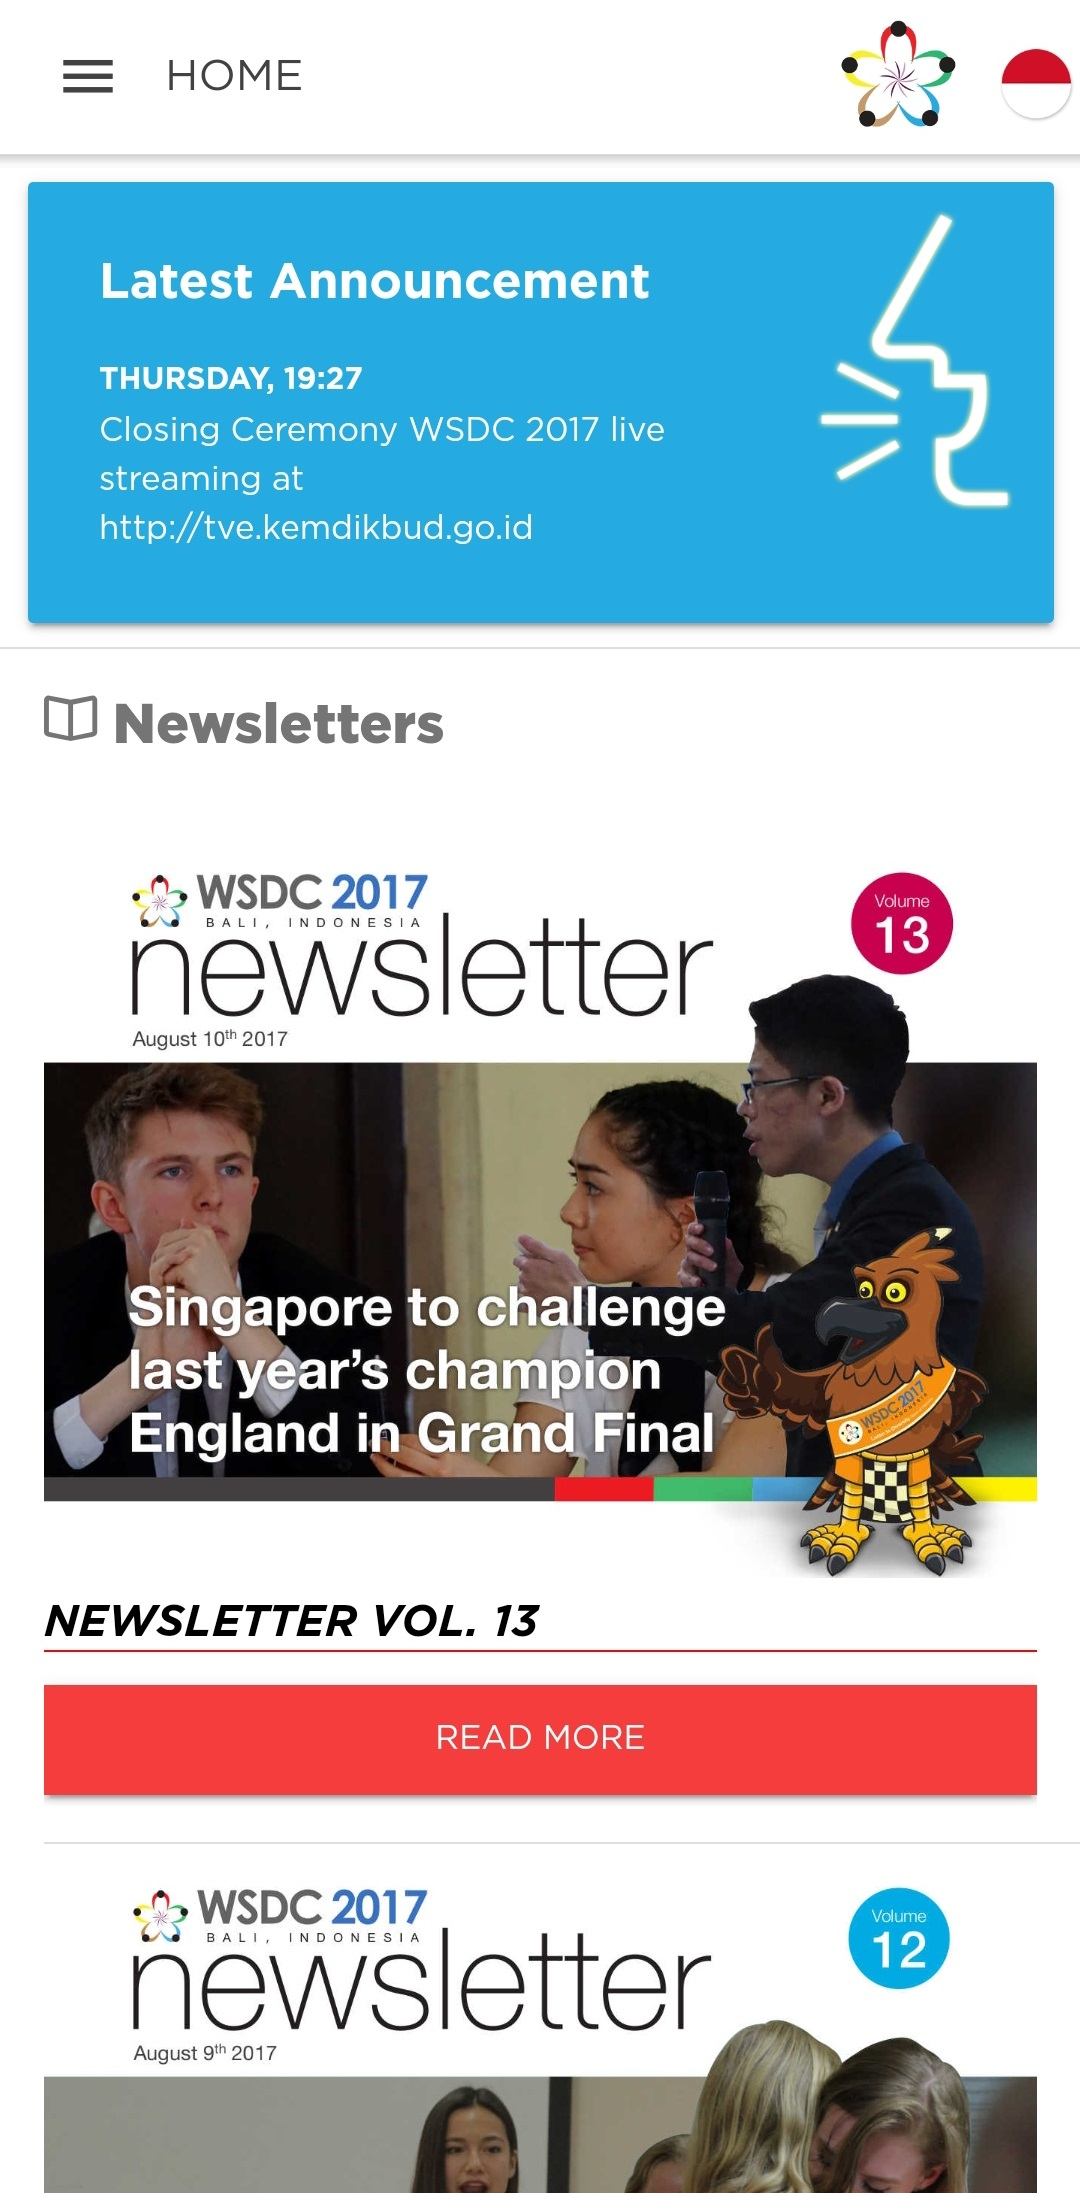
\includegraphics[scale=0.12]{Gambar/WSDC2017-App.jpg}
    \caption{Halaman utama aplikasi WSDC 2017 Bali pada Perangkat Android}
    \label{fig:wsdcapp}
\end{figure}
\newpage
Fitur-fitur yang terdapat di aplikasi WSDC 2017 Bali saat ini yaitu :

\begin{enumerate}
	\item {\it Announcements} : Pengguna dapat melihat pemberitahuan tentang berjalannya acara WSDC 2017 Bali.

	\begin{figure}[H]
	    \centering
	    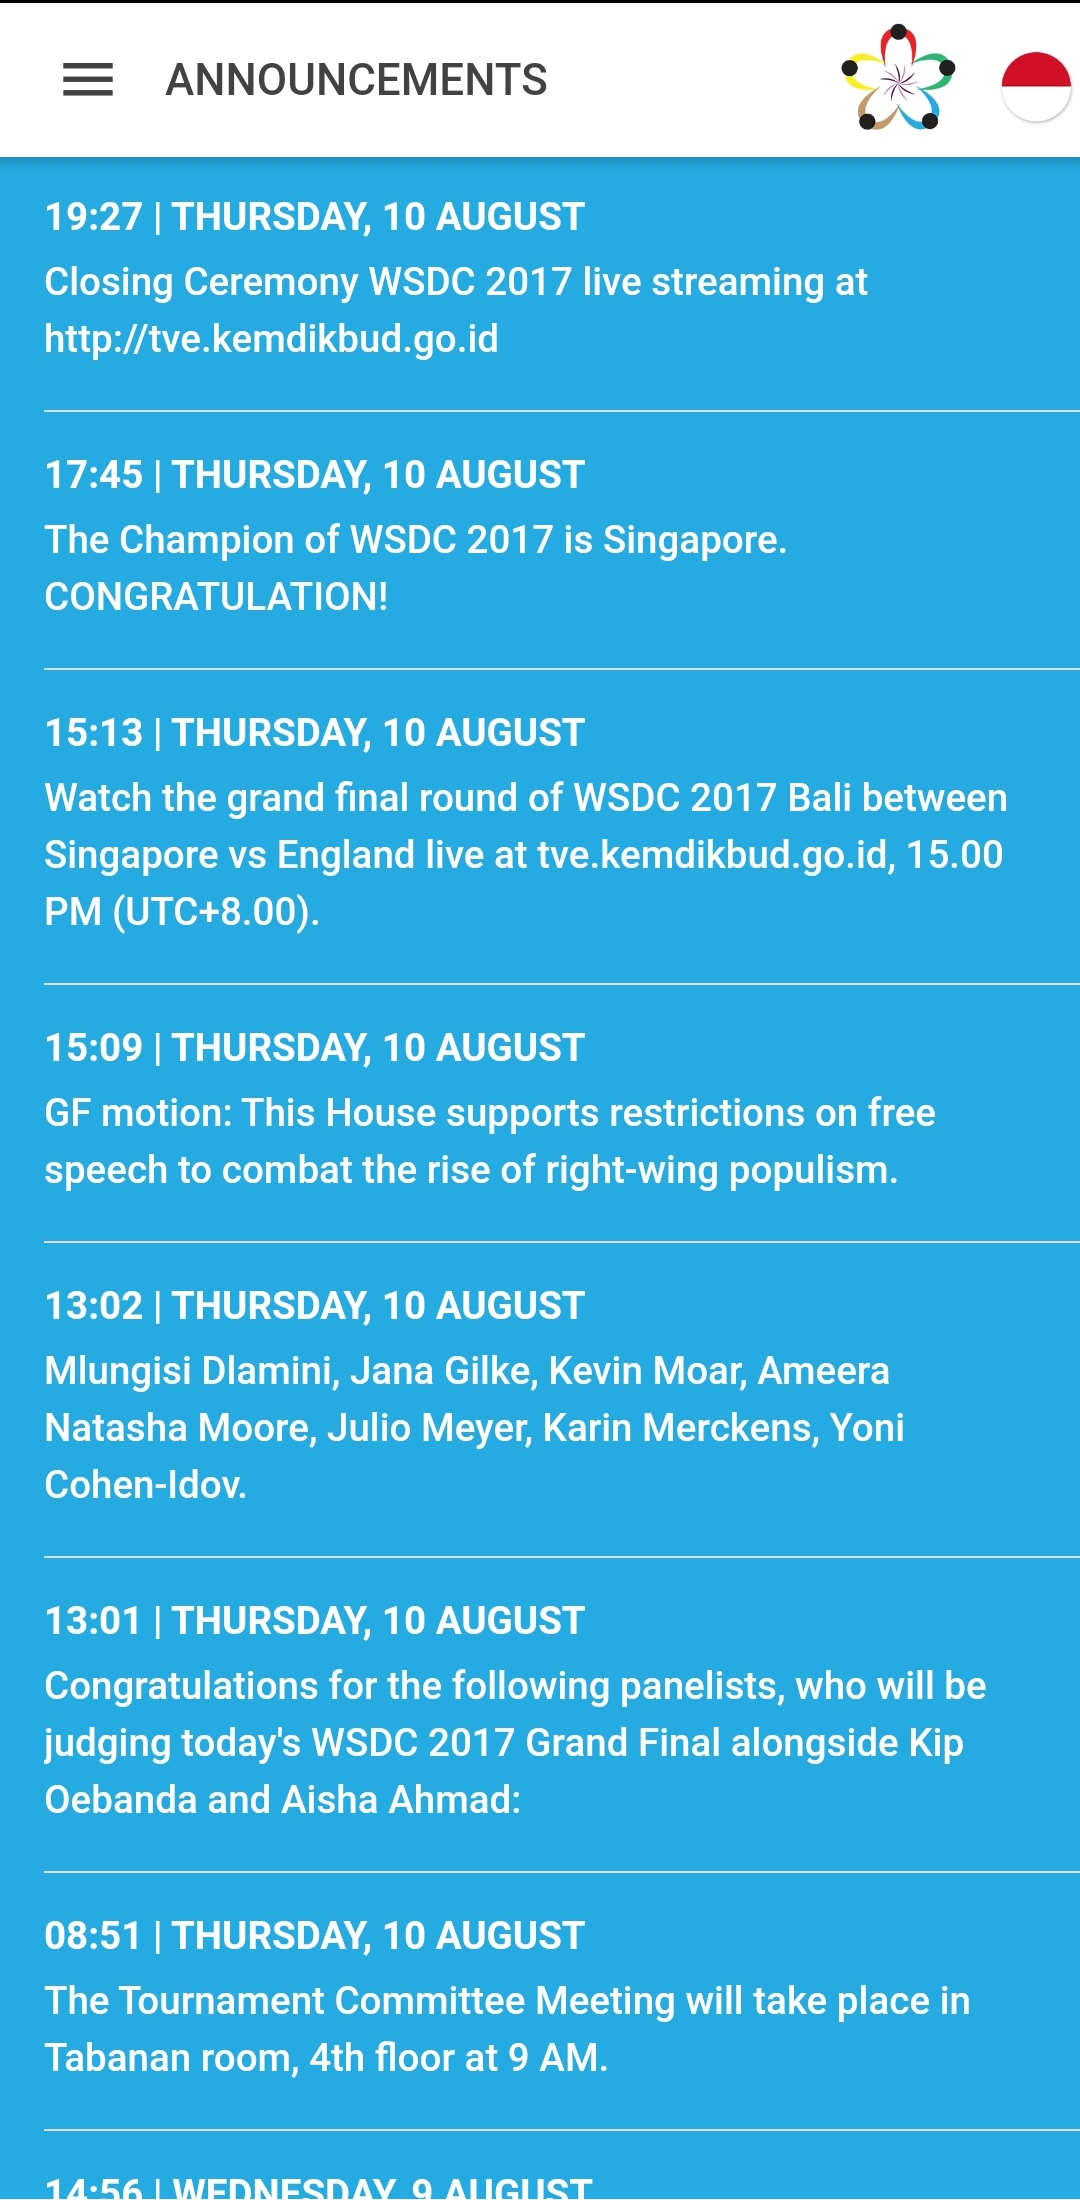
\includegraphics[scale=0.12]{Gambar/Announcements.jpg}
	    \caption{Halaman {\it Announcements} aplikasi WSDC 2017 Bali pada Perangkat Android}
	    \label{fig:wsdcappannouncements}
	\end{figure}

	\item {\it Schedule} : Pengguna atau peserta WSDC 2017 Bali dapat melihat jadwal acara yang sudah diadakan.

	\begin{figure}[H]
	    \centering
	    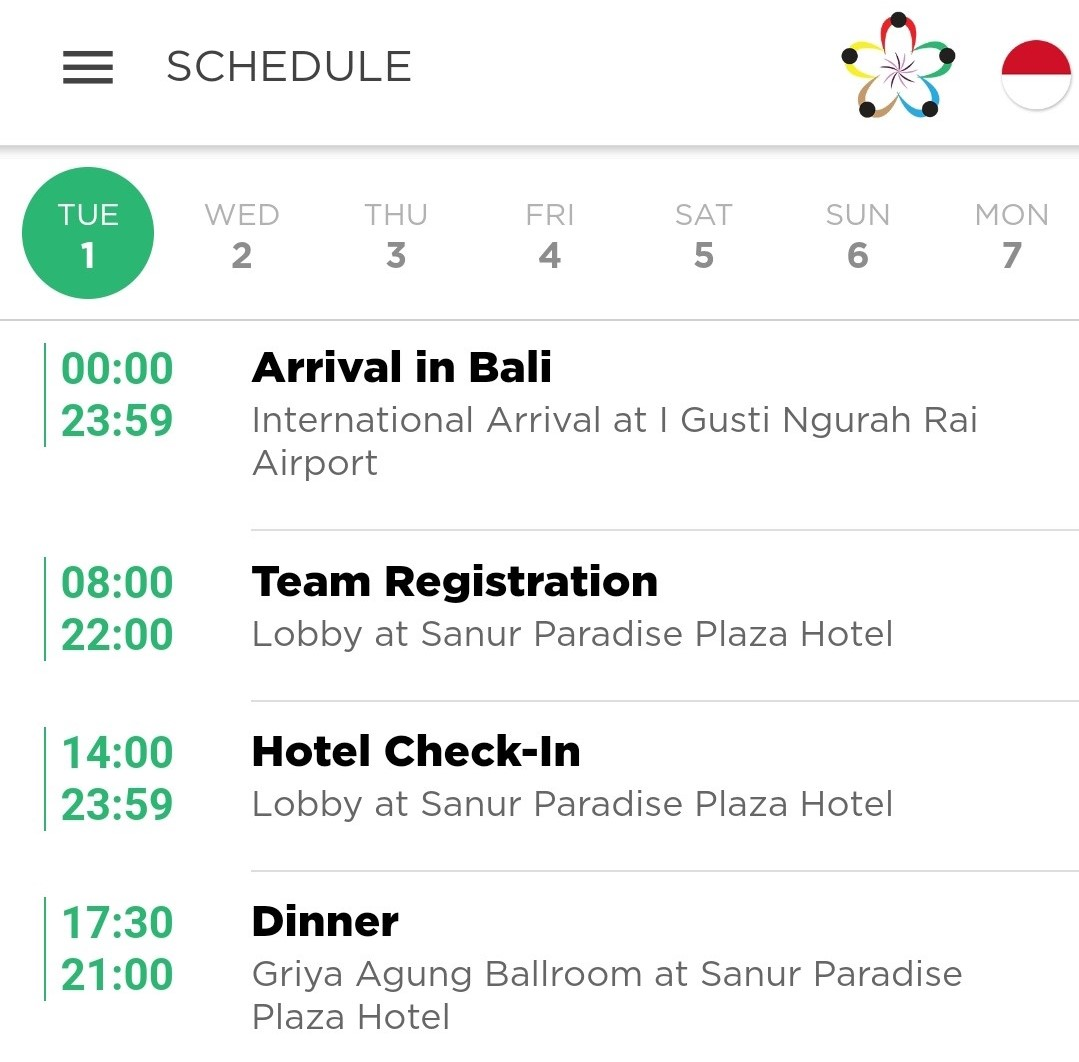
\includegraphics[scale=0.3]{Gambar/Schedule.jpg}
	    \caption{Halaman {\it Schedule} aplikasi WSDC 2017 Bali pada Perangkat Android}
	    \label{fig:wsdcappschedule}
	\end{figure}

\newpage

	\item {\it Venues} : Pengguna atau peserta WSDC 2017 Bali dapat melihat berbagai macam lokasi acara, mulai dari lokasi upacara, lokasi kompetisi, dan lokasi wisata edukasi. Masing-masing dari lokasi tersebut dapat menunjukan arah dan jarak dari lokasi tempat pengguna berada.

	\begin{figure}[H]
	    \centering
	    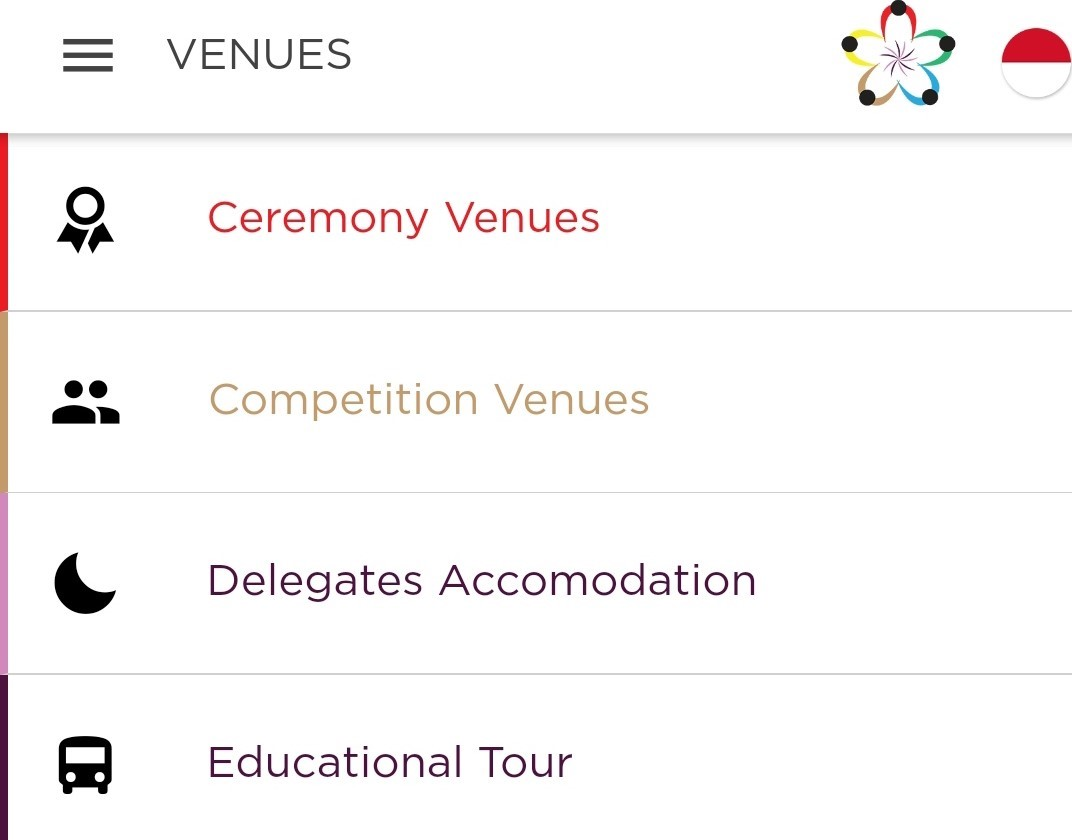
\includegraphics[scale=0.3]{Gambar/Venues.jpg}
	    \caption{Halaman {\it Venues} aplikasi WSDC 2017 Bali pada Perangkat Android}
	    \label{fig:wsdcappvenues}
	\end{figure}

	\item Info : Pengguna dapat melihat informasi terkait dengan tim pengembang dari aplikasi WSDC 2017 Bali, kontak-kontak penting yang dapat dihubungi, dan kosa kata penting dalam Bahasa Indonesia.

	\begin{figure}[H]
	    \centering
	    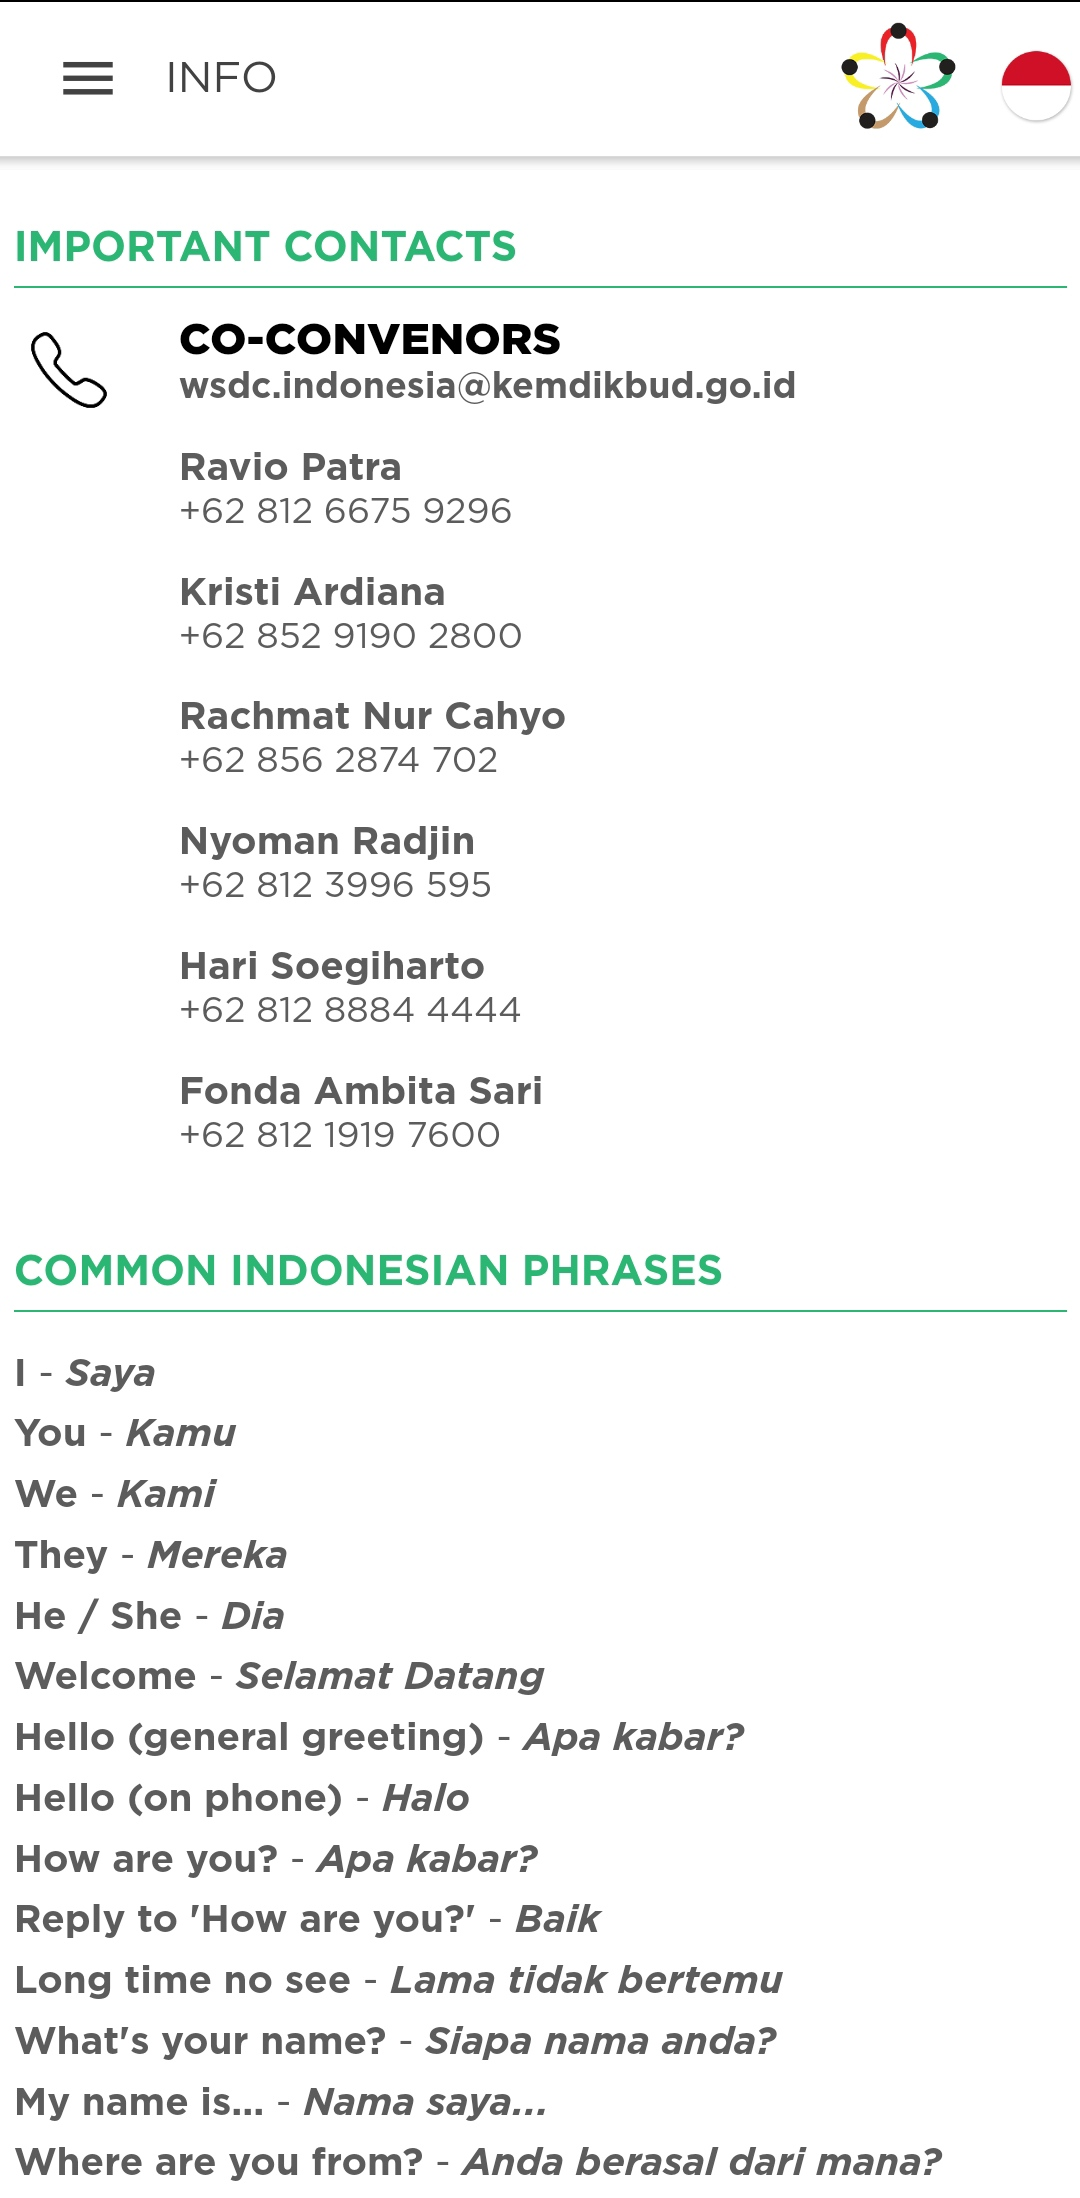
\includegraphics[scale=0.12]{Gambar/Info.jpg}
	    \caption{Halaman Info Aplikasi WSDC 2017 Bali pada Perangkat Android}
	    \label{fig:wsdcappinfo}
	\end{figure}
\end{enumerate}

\section{Ionic}
\label{sec:ionic} 
 
Ionic merupakan sebuah kerangka kerja {\it open source} lintas platform yang memungkinkan untuk mengembangkan aplikasi hibrida yang bekerja pada berbagai macam platform seluler seperti {\it android}, iOS, dan Windows~\cite{waranashiwar:18:ionic}. Ionic memiliki berbagai macam \textit{front-end library} dan \textit{User Interface}(UI) {\it Components} yang digunakan untuk  perancangan aplikasi menggunakan teknologi web seperti HTML, CSS, dan Javascript, dengan integrasi untuk berbagai \textit{framework} seperti Angular, React, dan Vue. Saat pertama kali dibuat, Ionic menggunakan AngularJS. Namun, seiring saat Angular versi 2 yang menggunakan Typescript dirilis, Ionic versi 2 dan selanjutnya menggunakan Angular. Lalu, pada tahun 2019, Ionic mendukung penggunaan \textit{framework} lain selain Angular, yaitu React dan Vue.

Pada skripsi ini akan menggunakan {\it framework} Angular. Versi Angular yang terpasang pada aplikasi WSDC 2017 Bali saat ini adalah versi 4.1.3. Sedangkan pada skripsi ini akan menggunakan Angular versi 12.  Di dalam Ionic, Angular digunakan untuk membangun aplikasi dan perutean, sehingga aplikasi dapat sejalan dengan ekosistem Angular lainnya. Ionic menyediakan @ionic/angular-toolkit untuk membangun aplikasi dan terintegrasi dengan Angular CLI resmi yang menyediakan fitur yang khusus untuk aplikasi @ionic/angular.

%\subsection{Instalasi}
%\label{subsec:instalasi}
%Aplikasi Ionic dibuat dan dikembangkan melalui perintah {\it command-line}. Pada skripsi ini akan melakukan penginstalan melalui metode Ionic CLI, yang akan menjadi alat utama untuk menjalankan aplikasi. Langkah-langkah instalasi Ionic CLI yaitu :
%\begin{enumerate}
	%\item Instalasi Node.js \\
	%Sebelum memulai instalasi Ionic, diperlukan penginstalan Node.js pada komputer. 
%\end{enumerate}

\subsection{Migrasi Ionic 3 ke Ionic 5}
\label{subsec:migrasi}
%Aplikasi WSDC Bali 2017 saat ini menggunakan {\it framework} Ionic versi 3 yang sudah tidak didukung lagi. Maka dari itu dilakukan pembaruan aplikasi WSDC 2017 Bali ke dalam {\it framework} Ionic versi 5. 

Untuk melakukan migrasi dari Ionic 3 ke Ionic 5 memerlukan dua tahap, yaitu migrasi dari Ionic 3 ke Ionic 4, dan migrasi Ionic 4 ke Ionic 5. Migrasi tersebut adalah sebagai berikut:

\begin{enumerate}
	\item Migrasi Ionic 3 ke Ionic 4 \\
	Ada beberapa langkah untuk melakukan migrasi dari Ionic 3 ke dalam Ionic 4, yaitu:
	
	\begin{enumerate}
		\item Membuat Projek Baru \\
		Langkah-langkah untuk membuat projek Ionic baru antara lain :
		\begin{enumerate}
			\item Ionic Start \\
			Untuk membuat projek baru menggunakan {\it Command Line} Windows, dengan mengetikan perintah \textbf{ionic start WSDC}.
			\item Memilih {\it Framework} \\
			Setelah itu akan ada pilihan untuk memilih {\it framework} yang akan digunakan (Gambar \ref{fig:memilihframework}). Pada skripsi ini akan menggunakan {\it framework} Angular.
			\begin{figure}[H]
			    \centering
			    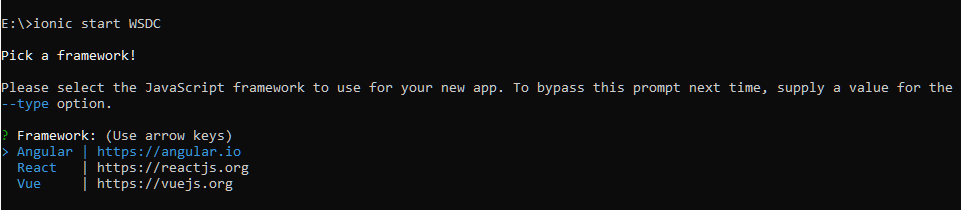
\includegraphics[scale=0.6]{Gambar/ssmemilhframework.png}
			    \caption{Pemilihan {\it template} Pada Command Line}
			    \label{fig:memilihframework}
			\end{figure}			
			\newpage
			\item Memilih {\it Template} \\
			Lalu setelah itu ada pemilihan {\it template} untuk memilih {\it template} awal yang akan digunakan (Gambar \ref{fig:memilihtemplate}). Pada skripsi ini untuk {\it template} awal akan menggunakan {\it blank}.
			\begin{figure}[H]
			    \centering
			    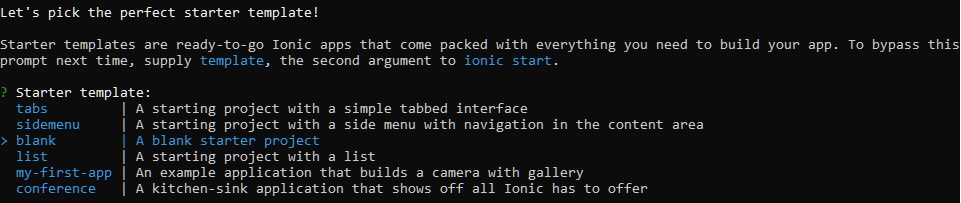
\includegraphics[scale=0.6]{Gambar/ssmemilihtemplate.png}
			    \caption{Pemilihan {\it template} Pada Command Line}
			    \label{fig:memilihtemplate}
			\end{figure}
			\item Memasang {\it Dependencies} \\
			Akan ada proses mengunduh berkas {\it dependencies framework} Ionic dan memasangnya di komputer (Gambar \ref{fig:ssunduhinstalionic}). Setelah proses pengunduhan dan pemasangan selesai, projek Ionic baru sudah dapat digunakan sepenuhnya.
			\begin{figure}[H]
			    \centering
			    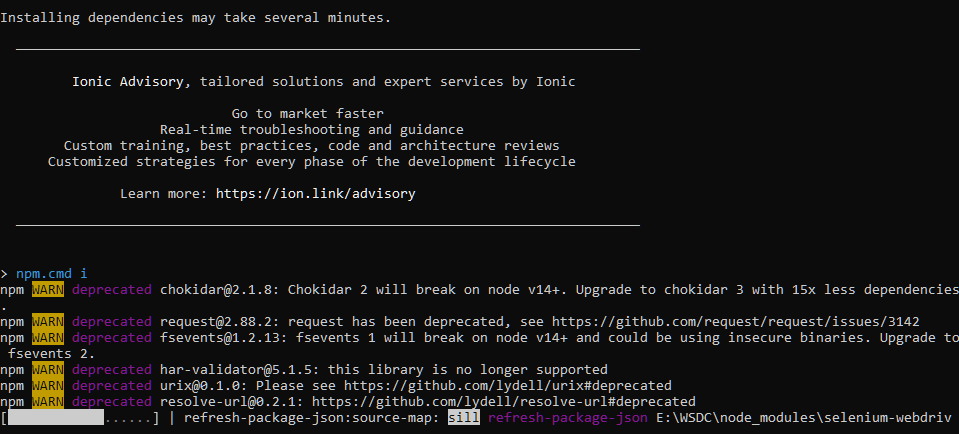
\includegraphics[scale=0.6]{Gambar/ssunduhinstalionic.png}
			    \caption{Proses Pengunduhan dan Instalasi {\it Dependencies} Ionic}
			    \label{fig:ssunduhinstalionic}
			\end{figure}
		\end{enumerate}
		\item Menyalin {\it Root-level Items} \\
		Menyalin seluruh {\it Root-level Items} pada Ionic versi 3 dengan direktori yang sama atau dengan beberapa perubahan. Terdapat beberapa perubahan baik itu nama maupun letak dari suatu fungsi atau berkas. Perubahan tersebut yaitu:
		\begin{itemize}
			\item Angular
			\begin{itemize}
				\item HttpClient \\
				Pada Angular versi 4 keatas, objek {\it response} secara {\it default} merupakan JSON, jadi tidak perlu dirubah kembali menjadi JSON.
			\end{itemize}
			\newpage
			\item {\it Imports}
			Terjadi perubahaan dalam mengimpor {\it package} di Ionic 3 dan Ionic 4. Daftar perubahan tersebut adalah sebagai berikut :
			\begin{itemize}
				\item Angular HTTP \\
				Ionic 3 : @angular/http\\
				Ionic 4 : @angular/common/http
	
				\item Ionic Angular \\
				Ionic 3 : ionic-angular  \\
				Ionic 4 : @ionic/angular
	
				\item {\it In App Browser} \\
				Ionic 3 : @ionic-native/in-app-browser \\
				Ionic 4 : @ionic-native/in-app-browser/ngx
			\end{itemize}
	
			\item Ionic {\it Component}
			Terjadi perubahaan pada Ionic {\it Component} di Ionic 3 dan Ionic 4. Daftar perubahan tersebut adalah sebagai berikut :
			\begin{itemize}
				\item {\it Button} \\
				Ionic 3 : <button>  \\
				Ionic 4 : <ion-button>
			\end{itemize}
	
			\item Perbedaan Direktori Berkas \\
			Terjadi perubahaan direktori pada berkas di Ionic 3 dan Ionic 4. Daftar perubahan tersebut adalah sebagai berikut :
			\begin{itemize}
				\item {\it Global Styling} \\
				Ionic 3 : src/app/app.scss \\
				Ionic 4 : src/global.scss

				\item {\it Pages} \\
				Ionic 3 : src/pages  \\
				Ionic 4 : src/app/pages
			\end{itemize}
	
			\item Penamaan Berkas
			Terjadi perubahaan penamaan pada berkas di Ionic 3 dan Ionic 4. Daftar perubahan tersebut adalah sebagai berikut:
			\begin{itemize}
				\item {\it Page} \\
				Contoh perbedaan nama {\it file} pada folder Pages adalah sebagai berikut :\\
				Ionic 3 : home.html  \\
				Ionic 4 : home.page.html
	
				\item {\it App} \\
				Contoh perbedaan nama {\it file} pada direktori App adalah sebagai berikut : \\
				Ionic 3 : app.html \\
				Ionic 4 : app-component.html
			\end{itemize}

			\item {\it Routing}
			\begin{itemize}
				\item {\it Selector} \\
				Contoh perbedaan {\it selector} pada halaman Home adalah sebagai berikut :\\
				Ionic 3 : page-home  \\
				Ionic 4 : app-home
			\end{itemize}
			
		\end{itemize}
		\newpage
		\item Menyalin Bagian-bagian Aplikasi \\
		Menyalin keseluruhan bagian yang ada pada aplikasi WSDC 2017 Bali, baik itu halaman maupun fitur yang ada, dengan ketentuan sebagai berikut :
		\begin{itemize}
			\item Shadow DOM sudah aktif secara {\it default}.
			\item Halaman atau komponen Sass tidak lagi dibungkus dengan tag halaman / komponen dan harus menggunakan opsi styleUrls milik Angular dari dekorator @Component.
			\item RxJS \\
			Pada Ionic 3, RxJS yang digunakan adalah versi 5. Sedangkan pada Ionic 4, RxJS yang digunakan adalah versi 6. Terdapat beberapa perbedaan diantara kedua versi tersebut, diantaranya yaitu :
			\begin{itemize}
				\item {\it Operator} \\
				Dalam pemanggilan operator, sejak RxJS versi 6 perlu menambahkan .pipe untuk menggunakan operator apapun.
			\end{itemize}
			\item {\it Lifecycle Hooks} tertentu harus digantikan dengan Angular Hooks.
		\end{itemize}
	\end{enumerate}
	\item Migrasi Ionic 4 ke Ionic 5 \\
	Migrasi aplikasi dari Ionic 4 ke Ionic 5 memerlukan beberapa pembaruan mengenai properti API, CSS, dan {\it package} dan {\it dependencies} yang terpasang. Perubahan-perubahan tersebut yaitu :
	\begin{itemize}
		\item API
		\begin{itemize}
			\item {\it Component}
			%\begin{itemize}
				%\item {\it Button} \\
				%Terjadi perubahan penulisan pada kelas activated, dari \textbf{.activated} di Ionic 4 menjadi \textbf{.ion-activated}.
			%\end{itemize}
			\item {\it Color}
			
		\end{itemize}
		\item CSS \\
		
		\item {\it Package} dan {\it Dependencies} \\
		Pada skripsi ini, aplikasi menggunakan {\it framework} Angular. Untuk melakukan pembaruan terhadap {\it package} dan {\it dependencies} terbaru, dapat dilakukan dengan cara menjalankan \textbf{npm install @ionic/angular@latest @ionic/angular-toolkit@latest --save} pada {\it command line}.
	\end{itemize}
\end{enumerate}

\subsection{Cordova}
\label{subsec:cordova}
Cordova merupakan {\it framework open source} yang dapat membuat pengembang untuk menggunakan teknologi seperti HTML, JavaScript, dan CSS untuk membangun aplikasi untuk perangkat bergerak yang dapat berjalan pada beberapa sistem operasi {\it mobile}~\cite{gonsalves:18:evaluating}. {\it Framework} Ionic digunakan bersamaan dengan Cordova untuk mengembangkan aplikasi WSDC 2017 Bali. 

%3 ke 4, 4 ke 5
%perubahan nama package
%bab 3 : 3 statusnya gimana, gabisa dijalanin karena apa, errornya gimana, 
%bab 2 : migrasi, actual migrationnya yg dipraktekan yg dikerjakan
%bab 2 : dasar teori, bahas wsdc app, ionic nya sendiri,
%bab 3 dan 4 : mengira ngira apa saja yg akan dikerjakan dari dasar dasar di bab 2
%



